\chapter{Watermarking}
\Gls{watermarking} is cool! Le ssw aussi\cite{cox1997secure}
\section{Presentation}
\section{Existing work}
\section{Techniques}
\subsection{Least Significant Bit}
\subsection{Spread-spectrum Watermarking}

The purpose of the spread-spectrum watermarking (SSW) method is to embed the hidden data of the watermark in the frequency domain of the host signal. Hence, SSW algorithm relies on a time-to-frequency transform and on its inverse transform. In fact, any frequency transform can be used with this method, as long as the same transform is used for watermarking insertion and detection. For example, in this project, we used the Discrete Fourier Transform.

~

The core of this method is based on a random sequence of N numbers, whose values are either $1$ or $-1$, with a equal distribution for both. This sequence is the key of decryption and thus must be known by the emitter and the receiver.

~

Therefore, the first step is to generate this sequence.

\subsubsection{Watermark insertion}

In order to embed data with the SSW method, the host signal must firstly be divided into chunks of given size (for example, chunks of $512$ samples). The SSW algorithm can then be applied to each of these chunks in order to embed the hidden data. Only 1 bit of hidden data can be embedded in a chunk.

~

On each chunk, the frequency transform is then applied. The result is an array of half the size of the chunks, each cell of it containing the energy and phase for a certain frequency bin of this chunk.

~

The next step is to select N (the size of the random sequence) frequency bins that are going to be modified. Therefore, N has to be less than half the chunk size. The goal is to avoid inaudible portions of the frequency spectrum because they are more likely to create audible noise when modified. The best is to keep frequency bins in the $200$ Hz - $2$ kHz subband.

~

Let's call $F$ the sequence of the magnitudes (in decibels) of the selected frequency bins and $S$ the random sequence. The following is then performed :

~

$F[i] = F[i] + W[k] \times \delta \times S[i]$, for $i$ varying from 1 to N.

~

\noindent where $W$ is the hidden data to be embedded ($W[k]$ is equal to 1 for bit 1 and -1 for bit 0), $k$ the current bit of hidden data and $\delta$ the amplitude of the watermark (usually between $0.5$ and $2.5$ dB).

~

After the modification on the frequency magnitudes, the time signal is reconstructed using the original phases and the inverse frequency transform.

\subsubsection{Watermark detection}

Just like in the embedding part, the signal must be divided into chunks. They have to be the same size as during embedding.

~

The frequency transform is also applied and the same frequency bins as before are also selected. Magnitudes in decibels are computed as well but instead of modifying them, a correlation is calculated, just as follows :

~

$C = F \cdot \delta S$

~

\noindent where $F$ is the sequence of selected frequencies magnitudes, $S$ the random sequence and $\cdot$ the normalized dot product.

~

When the chunk has not been watermarked, $C$ should be close to $0$ because $F$ would be close to a random sequence, and when the chunk is watermarked, $C$ should be closer to $1$ because $F$ would be equal to $random + \delta S$ and $\delta S \cdot \delta S = 1$. When the bit 0 is embedded, $F$ is equal to $random - \delta S$, so $C$ should be closer to $-1$.

~

Hence, for each chunk, it is possible to determine whether or not there is a watermark (by using a threshold) and if so, which bit of data is embedded. Doing it for each chunk allows for the reconstruction of the entire hidden data.

~

A bigger $N$ would allow better correlation values but also a more audible watermark. The same rule applies to $\delta$.

~

There are several methods that can improve watermark detection, like cepstrum filtering, but these were not implemented in this project.

\subsection{Compression-Expansion}\cite{foo2010}

Compression-expansion is a time-based method for watermarking, unlike S.S.W. which is a spectral-based method.\\
Its purpose is based on dividing a signal into segments of frames that overlap each other, calculate a local mask and taking specific coefficients according to the mask previously calculated from a frame to add them to the end of the following one. The technique is detailed in this subsection.

\paragraph{Purpose of the compression-expansion of segments}
Let's consider a signal. One divide it into segments that are containing the same number of frames.\\
The division must be in respect of the following purpose : each segment half-overlaps the following one. A Hanning window is then applied to the segments, as showed by the following figure :
\begin{figure}[H]
\center{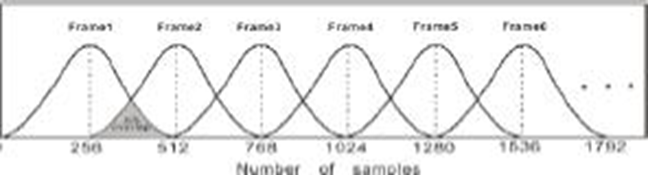
\includegraphics{images/Image1.png}}
\caption{\label{frames} Division into frames of a signal}
\end{figure}
For each bit of the watermark, two segments are used. So that no confusion is made, the third segment that follows the two segments used is left.\\
A discret cosine transform (D.C.T.) is applied on the two segments that are under consideration. Here is used a local auditory mask, which is calculated thanks to a psychoacoustic model. We will see later how this mask is calculated.

According to the mask, in the first segment, one takes the 8 first coefficients of the D.C.T. that are greater than the mask. One must look for those coefficients from the end of the segment. As one has removed coefficients from a segment, it is compressed\\
Those coefficients are then added to the beginning of the following segment. It is thus expanded.\\
The following figure sums up this operation :
\begin{figure}[H]
\center{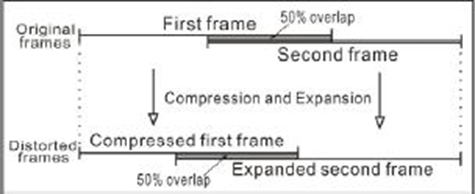
\includegraphics{images/Image2.png}}
\caption{\label{compression-expansion} Compression and expansion of the segments}
\end{figure}

An inverse D.C.T. is applied then to come back to the time domain. The differences between the original signal and the reconstructed one yields a signal made up of little waveforms that have the shape of a diamond, such as this figure shows :
\begin{figure}[H]
\center{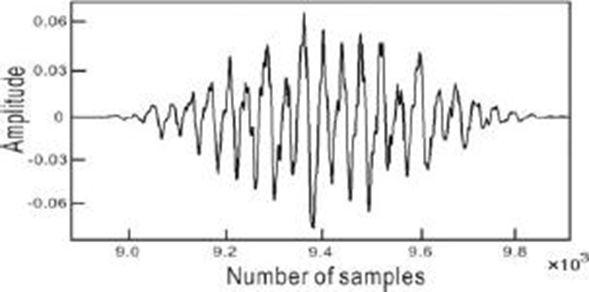
\includegraphics{images/Image3.png}}
\caption{\label{diamond} Diamond obtained by the difference of original and reconstructed waveforms}
\end{figure}

\paragraph{Use of the diamonds}
Depending on the original signal, either mono, either stereo, the method differs. In each case, the diamonds that are previously obtained by the difference of the original signal and the reconstructed one are used, but in different ways.

Let's consider a mono signal. The principle is here to obtain a diamond to embed the bit "1" (therefore, apply the method described in the previous paragraph), and nothing to embed the bit "0" (no calculation).\\
As it is not sure that the processing of this type of watermarking begins exactly at the beginning of the signal, one must know where's the first bit embedded. One considers then that, when the encoding begins, a diamond is calculated.

For a stereo signal, one uses the two channels. On the left channel, a diamond is calculated to embed "1", and the other way round for "0" (on the right channel). The two channels enables the fact that there can be blanks on both channels at the same time, therefore having different time intervals between the diamonds.
\begin{figure}[H]
\center{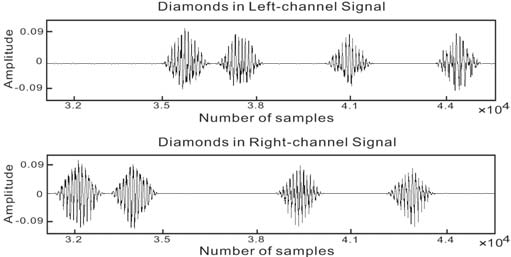
\includegraphics{images/Image5.png}}
\caption{\label{stereo watermarking} Series of diamonds for a stereo signal}
\end{figure}

The next step is to detect those diamonds. The main problem generated by the compression-expansion is that, in some cases, the distortion can be difficult to detect (the diamonds are to tiny), as this is showed in this figure :
\begin{figure}[H]
\center{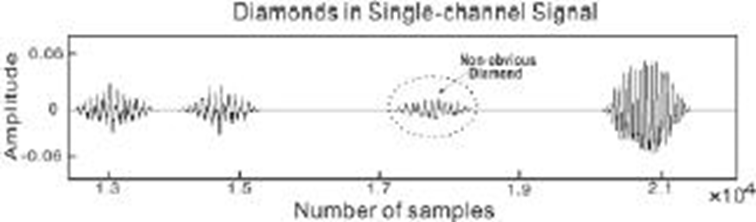
\includegraphics{images/Image4.png}}
\caption{\label{distortion} Example of a to much tiny diamond}
\end{figure}

Such a problem can be easily avoided in stereo signals, because the watermarks can be separated with blanks on both channels. But on a mono signal, if the diamond is considered as noise (therefore, not taken into consideration), it will yield a false detection of the watermark. This is a constraint for mono signals : some types of signals (such as those which encode speeches) can't be used to ensure a good accuracy. These types of signals have often parts where the energy is low, which means a low amplitude. As the diamond is obtained by taking the difference of the original signal and the reconstructed one, this difference is as low as the amplitude of the signal is weak.

To detect the watermark inside a signal, the original non-watermarked signal is needed to calculate the diamonds. The detection of the diamonds can be done with several methods : some are described here.\\
\begin{itemize}
\item \textbf{Sum of absolute difference} : one computes the sums of absolute differences between the watermarked signals and the original signals. So as to detect a diamond, which duration is equal to 2 segments of frames that overlap each other by 50\% in the signal, in addition to one frame unused due to the 50\% overlap, each sum is calculated on the base of 3 segments as described previously. On the one hand, when there is a diamond (thus, a distortion on the watermarked signal), the sum of the absolute values of the differences during the distortion is found to be greater than 5,5. On the other hand, the sum of the absolute values of the differences is always under 0,8. Thus, a threshold of $\frac{5,5 + 0,8}{2} = 3,15$ can be taken to detect a diamond.\\
This method is very simple and very accurate when no attack is done on the watermarked signal. But when it is damaged, several errors of detection can be made.
\item \textbf{Calculation of gradients} : a diamond has two slopes that make the shape of a triangle, such as showed on the figure below :
\begin{figure}[H]
\center{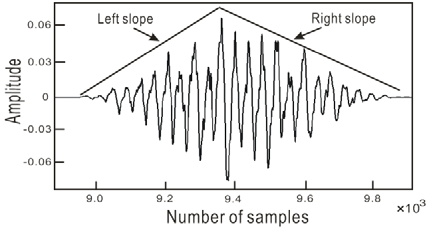
\includegraphics[scale=0.7]{images/Image6.png}}
\caption{\label{slopes} The slopes for a diamond}
\end{figure}
The derivative of each slope should be a constant non-zero function. It is experimentally found that the constant values of these function are greater than 1.7 for the left slope and lower than -1.5 for the right slope. These criteria can be used to ensure that the segments considered where used to calculate a diamond or not.\\
From the experience, this type of searching works well on attacked signals with noise and re-sampling. Nevertheless, the results are less satisfying when the watermarked signal is compressed using a low-pass filter or M.P. 3 algorithm.
\item \textbf{Cross-correlation with reference triangle} : 
\end{itemize}